\documentclass[letterpaper,12pt,peerreviewca,draftcls]{IEEEtran}
\usepackage{csm16}
\usepackage[margin=1in]{geometry}
\usepackage[nolists,nomarkers,tablesfirst]{endfloat} % put figures at end
\usepackage{amsmath} % for \eqref

% added for CSMAG only
\usepackage{url}
\usepackage{graphicx,xcolor}
\usepackage{verbatim}% http://ctan.org/pkg/verbatim
\makeatletter
\newcommand{\verbatimfont}[1]{\def\verbatim@font{#1}}%
\makeatother
\verbatimfont{\ttfamily\small}
\newcommand{\XX}[1]{{\bf XX #1 XX}}
\newcommand{\bi}{\begin{itemize}}\newcommand{\ei}{\end{itemize}}
\newcommand{\be}{\begin{equation}}\newcommand{\ee}{\end{equation}}
\newcommand{\bee}{\begin{enumerate}}\newcommand{\eee}{\end{enumerate}}
\newcommand{\bea}{\begin{eqnarray}}\newcommand{\eea}{\end{eqnarray}}
\newcommand{\beas}{\begin{eqnarray*}}\newcommand{\eeas}{\end{eqnarray*}}
\newcommand{\bc}{\begin{center}}\newcommand{\ec}{\end{center}}
%
\usepackage[left,pagewise]{lineno} 
\usepackage[english]{babel} 
\usepackage{blindtext}
% added for CSMAG only

\title{IEEE Control Systems Magazine\\
\Large Sample and authors’ guidelines for manuscript preparation}
\author{Jonathan P.\ How, Jeremy VanAntwerp, Richard Braatz,\\ Dennis Bernstein, and Tariq Samad\\
	POC: J.\ How (how.jonathan@gmail.com)\\ \today }

\newif\ifPDF \ifx\pdfoutput\undefined\PDFfalse \else\ifnum\pdfoutput > 0\PDFtrue \else\PDFfalse \fi \fi
\ifPDF 
\usepackage[pdftex, plainpages = false, colorlinks=true, linkcolor=black, citecolor = green!50!blue, urlcolor = blue, filecolor=black, pagebackref=false, hypertexnames=false,  pdfpagelabels ]{hyperref}
\fi

\begin{document}
\maketitle
\CSMsetup
\linenumbers \modulolinenumbers[2] % added for CSMAG only

IEEE Control Systems Magazine (CSM) articles are intended to inform the control engineering community of developments in specialized areas of control. Therefore, submissions must strive for high-quality exposition that explains the principal issues and challenges of their applications area. At least some of the introduction must be of a tutorial nature to introduce non-experts to the area of application. CSM papers are intended to be expository, which means that they explain things to nonexperts, assuming knowledge of control and systems theory at the graduate level. The opening section of the article can review the relevant literature. 
A sidebar can be used to survey the relevant literature. Sidebars are encouraged for self-contained digressions and tutorials.

\section{Preliminary Remarks}
\begin{itemize}
\item Do not include an abstract. % No abstract is needed or allowed.
\item Do not number sections.  Center and boldface all section headings, and left-align and boldface all subsection headings. For subsubsection headings, use left justified, not bold, regular size font, italics.
\item Do not use footnotes of any kind or for any purpose. %No footnotes are allowed or used in any article published in IEEE CSM.
\item Use margins that are 1 inch on all sides allowing for US-size paper (\verb!\usepackage[margin=1in]{geometry}!). 
\item Punctuate every equation correctly within the context of the surrounding sentence.
\item You can use Word or LaTex, but \textit{LaTex is preferred for articles with numerous equations}. 
A LaTex template is available \cite{LT}.
\item Be sure that your references adequately capture prior relevant research. List references in the order of citation in the text. Use a dynamic citation process (such as bibtex or endnote) so that the references can be re-sorted if needed.
\item CSM encourages attractive illustrations, figures, and photos.  
Be sure that every figure has a detailed, informative caption in the Magazine style (see Figure~\ref{fig1}). 
\end{itemize}


\subsection{Formatting Instructions}

In preparing your article for the IEEE Control Systems Magazine (CSM), please note the following guidelines concerning layout and formatting. Please order the elements of your manuscript as follows:  
\begin{enumerate}
\item Title and subtitle.
\item Author names, clearly indicating point-of-contact author (with email address) on page 1.
\item Main text, with no heading for the first section, which is assumed to be the introduction.
\item References, beginning on a new page.
\item Each figure on a separate page with its caption, using (a), (b), (c) for subfigures. See ``\nameref{FTC}'' for details on figure caption style. In the text the subfigures should referenced as: Figure 2(a) and (b).
\item Each table on a separate page with its caption.  See below for details on table caption style.
\item Each sidebar beginning on a new page followed by its figures and tables labeled Figure S1, Table S1.  See below for more details on numbering figures, tables, and equations in sidebars. Each sidebar must be mentioned in the main text and the sidebars should be arranged in the same order that they are referenced in the text. 
\item On the last page, include a short biography of each author, beginning on a new page. 
\end{enumerate}
Each of these elements is described in detail in the following.


\subsection{Title and Subtitle}
IEEE CSM titles are in two parts, typeset in the exact style below.
The title should use initial caps and no colon.
The subtitle is on a separate line (note that only the first word is capitalized).
The subtitle should describe the content of the article.
Please choose the title and subtitle carefully.  Here is an example
\bc
{\Huge Control of Quantum Systems} \\
{\Large Subatomic phenomena\\
with application to feedback systems}
\ec
No colons should be used in either the title or the subtitle.  Avoid using the same word in both the title and subtitle.

\subsection{Main Text}

In assembling the main text, pay careful attention to the order of topics as well as the sectioning.  Choose section and subsection headings to reflect the material and to serve as a roadmap for the reader.
Do not provide a section heading at the beginning of your article, which IEEE CSM assumes is the introduction.
You can use subsubsection headings if you wish, but be sure to use them carefully so the reader can follow the layout.
%
Please use this style for review purposes:
\bi
\item[] Section heads:  Centered, bold, large font \verb!\section{}!
\item[] Subsection headings:  Left justified, bold, regular size font \verb!\subsection{}!
\item[] Subsubsection headings:  Left justified, not bold, regular size font, italics \verb!\subsubsection{}!
\ei
An example can be treated as a subsection or subsubsection.

\subsection{Figures, Tables, and Captions} \label{FTC}
IEEE CSM requires a uniform style for figure and table captions that is intended to enhance the quality and appearance of articles. 
Be sure that every figure and table is well motivated and transmits an essential point in relation to the main ideas of the article.  
%
IEEE CSM uses a descriptive and informative style for figure and table captions that enhances the impact and appeal of figures.  You can think of a figure or table caption as a summary of what you would say if you were presenting the figure or table in a PowerPoint presentation.  

Each caption must be informative, interesting, and helpful.  The figure or table caption may provide a summary of the main points from the text.  In fact, repetition between the figure caption and text is encouraged.  A figure or table caption can also be used as a mini-tutorial for the reader.   These captions will greatly enhance your paper and the overall quality of IEEE CSM.

The general style is that the figure should not have a caption or label along the top. The axes are labeled, and a legend should be used. Multiple curves can be distinguished by color or dashes and dots. The caption below the figure includes a title and one or more sentences of pertinent information.
\bee
\item Avoid using acronyms in figures and figure captions so that the figure captions can be read independently of the text.  If an acronym appears in a figure, then please redefine the acronym in the figure caption.
\item Please be sure that every figure, table, and sidebar is cited in the main text.
\item Place all figures on separate pages at the end of the document, in accordance with the order described above.  IEEE places the figures at the appropriate place when your article is typeset. The LaTex package \verb!\usepackage[nomarkers]{endfloat}! will help..
\item Table captions should be equally informative and located above the table, as shown in Table~1.
\eee
It is the responsibility of the author to obtain copyright permission for all materials that are subject to copyright protection.  It is the author’s responsibility to obtain this permission prior to final acceptance of the manuscript.  You do not need to obtain copyright permission before you submit your article. Each relevant figure caption must include an explicit statement that permission has been given.  At the end of the figure caption, include a statement such as ``(With permission of Smith and Jones Publishers.)" or ``(Image courtesy of Technocontrol, Inc.)."

\noindent The suggested caption format is (see Figure~\ref{fig1}):\\[-3em]
\bc
\begin{minipage}[t]{6in}
	Figure 1. Title of the plot, not a sentence. Next, a sentence is given here to indicate the points that the figure is meant to highlight. Finally, you can include additional sentences to provide more detail about the meaning and importance of the figure. These sentences will greatly enhance the appeal of your article. (With the permission of Bodeplots, Inc.)
\end{minipage}
\ec

\begin{figure}[t]
\centering
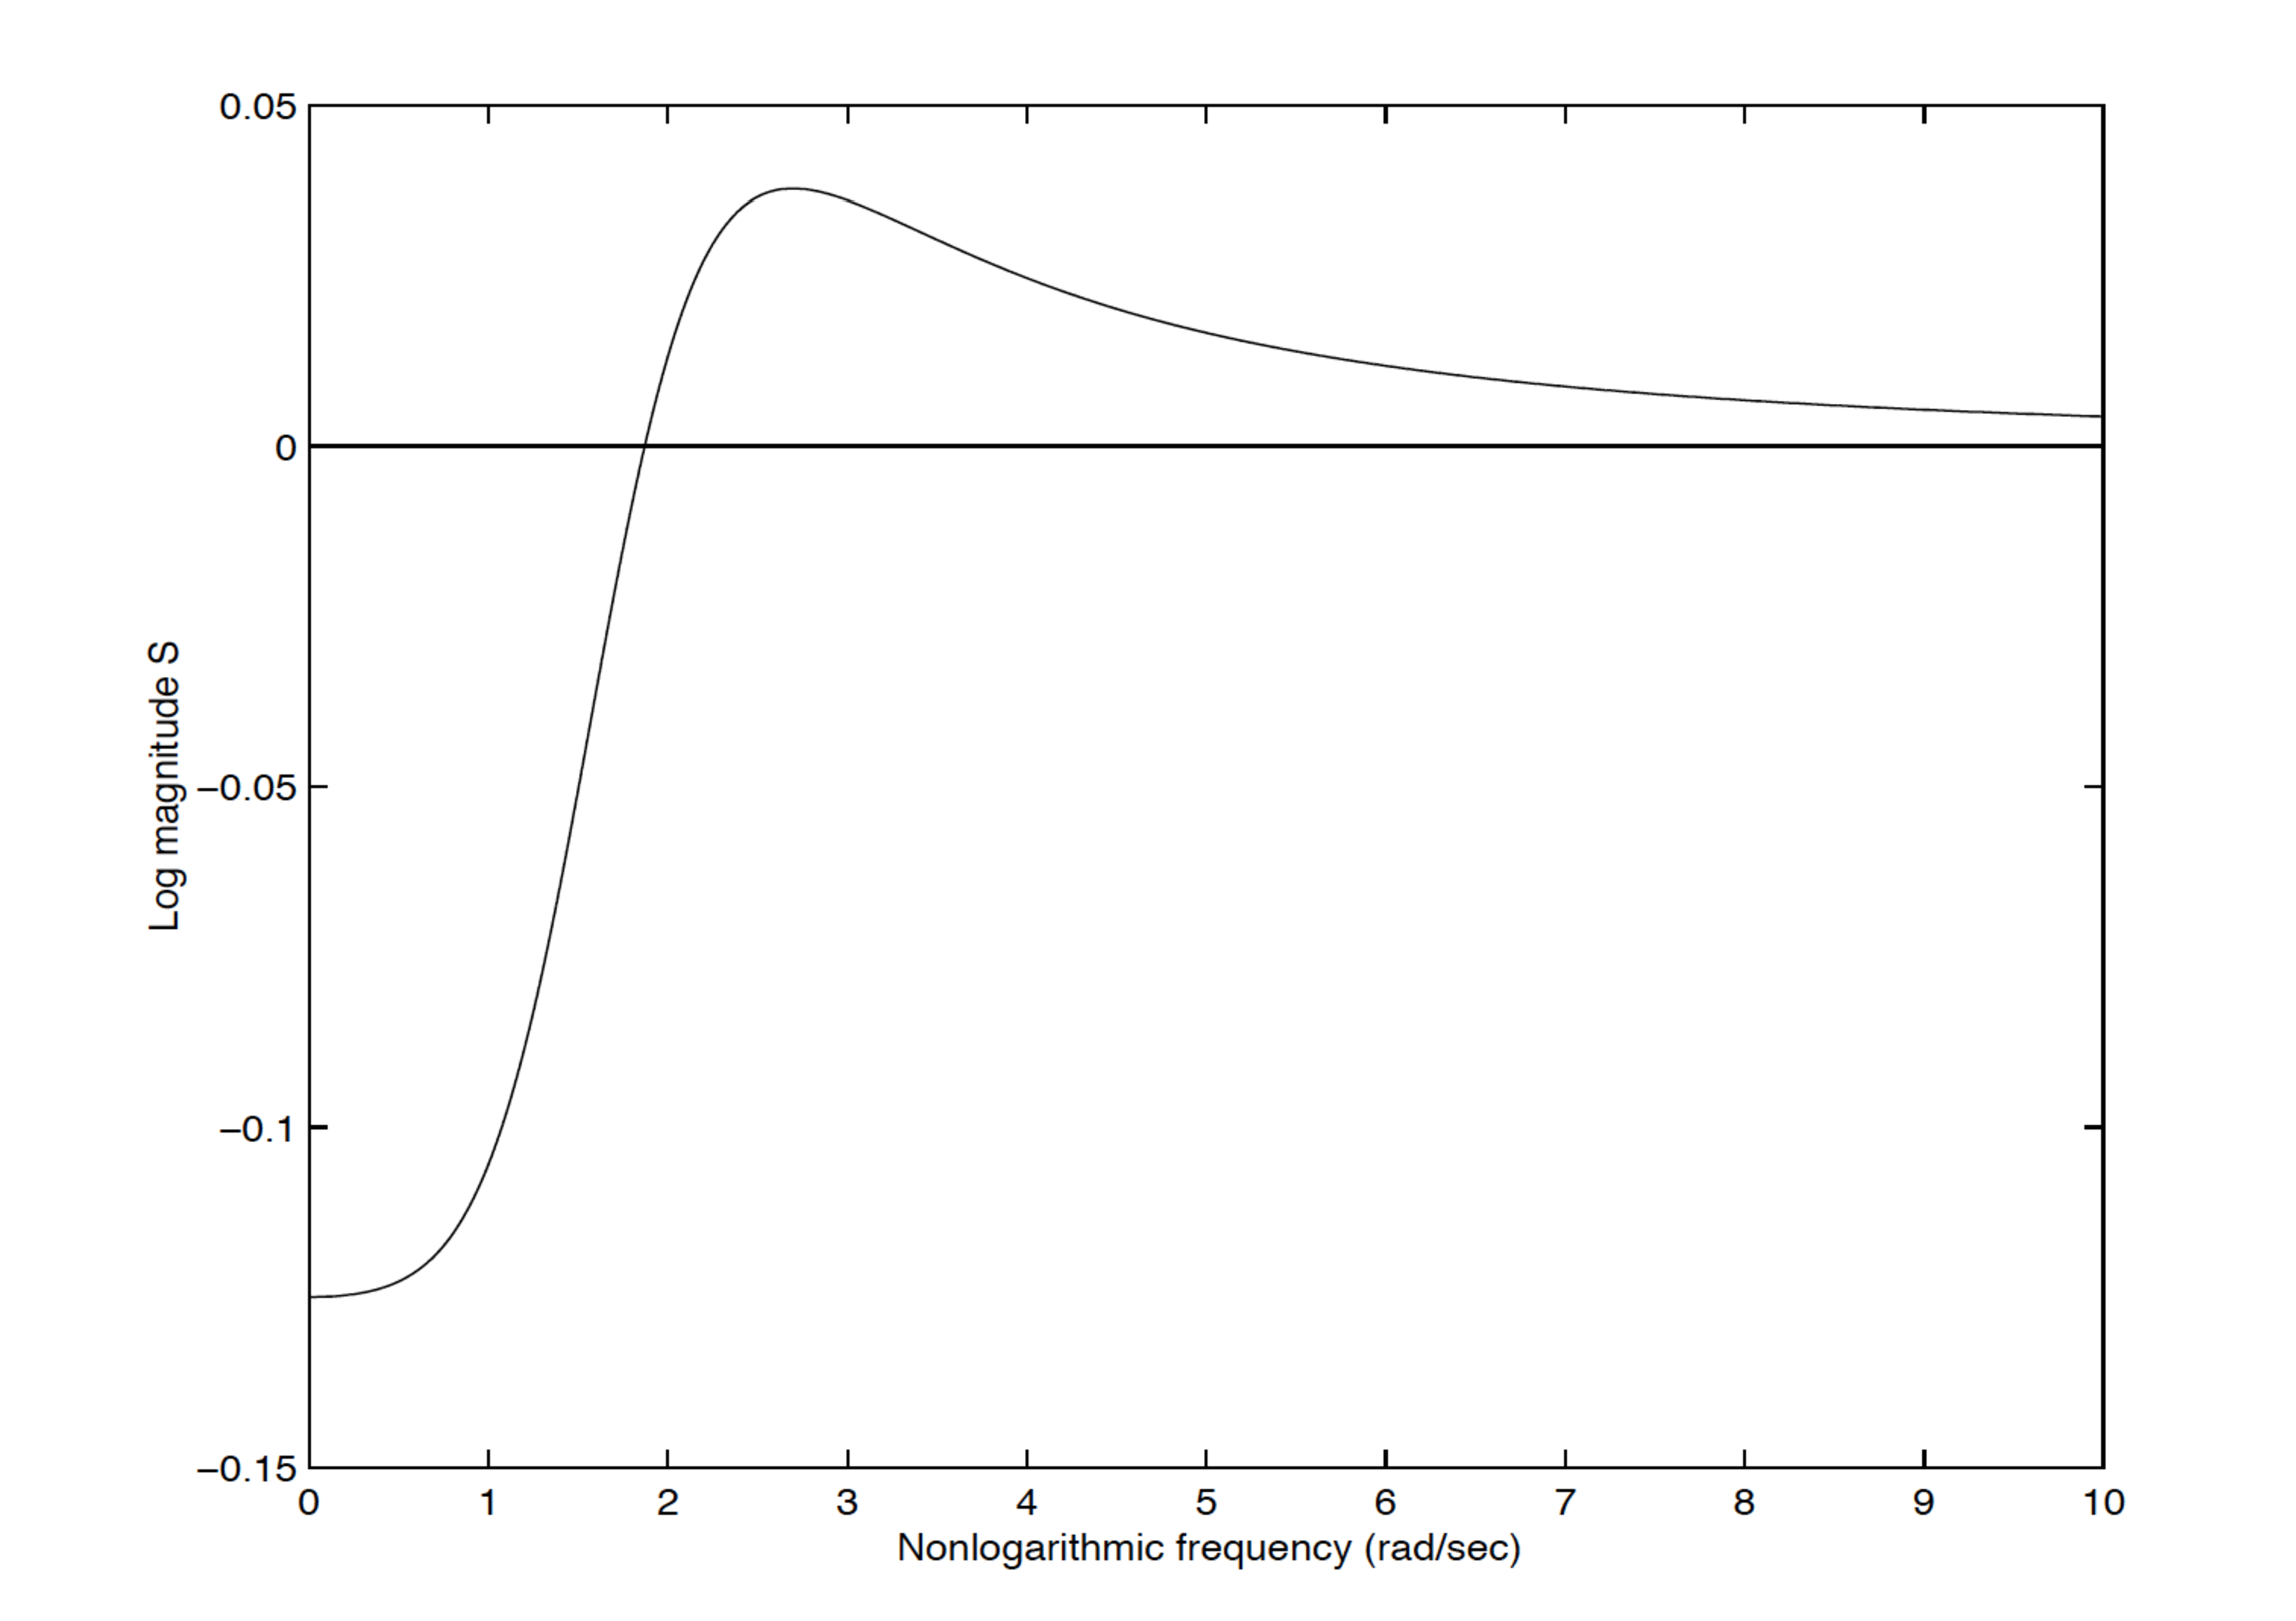
\includegraphics[width=0.85\textwidth,trim=10 10 10 10,clip]{figure1.pdf}
\caption{
	Bode plot of the sensitivity function. The negative and positive portions of the curve suggest that the benefits of feedback are accompanied by a cost of feedback. Analytical results show that these tradeoffs are inevitable for linear time-invariant systems whose relative degree is at least 2. Analogous results for multivariable and time-delay systems have been developed, but are not so well known. (Courtesy of Bodeplots, Inc.)}\label{fig1}
\end{figure}

\begin{table}[t] \caption{Compares the transient response to a step input for different architectures (cascade and two-input) of the dynamic output feedback controller with the same closed-loop poles locations. The full-state feedback (FSFB) result matches the predicted properties closely (limited by  the dominant pole pair assumption), but the cascade dynamic response is significantly different. The closed-loop response using the two-input dynamic output feedback controller discussed later closely matches the predicted values.} \vspace*{.1in}
	\centering
	\begin{tabular}{|l||c|c|c|c|} \hline 
		Property & Predicted & FSFB & Cascade & Two-input\\ \hline\hline
		Rise time (s) & 0.44 & 0.3798 & \textbf{0.1687} &0.4050\\
		Settling time (2\%) (s) &  0.9775 & 1.0534& 0.9593&1.0978\\
		%       SettlingMin& 0.9048& 0.9137&\\
		%      SettlingMax& 1.0432& 1.2799&\Ï\
		Overshoot (\%)& 4.0 & 4.3146& \textbf{27.9841}&3.9771\\
		%        Undershoot& 0& 0\\f
		%		        Peak& 1.0432& 1.2799\\
		Peak time (s) & 0.79 & 0.7873& \textbf{0.4648}&0.8459 \\ \hline
	\end{tabular}
\end{table}


\subsection{References}
All cited references must be publicly accessible.  Internal reports, theses, and dissertations are not viewed as being publicly accessible, and thus cannot be included in the reference list.  IEEE CSM is an archival publication, whose articles are backed up by other archival publications. However, obscure or unpublished documents that can be accessed from the web can be cited as long as the citation includes a URL address from which the document can be accessed.  In these cases, a website must be provided from which the document can be obtained.
All references need to be complete and accurately state the authors, title, volume, pages, and date.  Issue number is not crucial.

\subsubsection{Citation Style in the Text}
References must be listed in the order of citation in the text. Reference citations in the text must be bracketed numbers, that is, [3]-[5], [23]. For multiple nonsequential citations, separately bracket each number in numerical order, that is, [3], [5], [7].  In LaTex, the package 
\verb!\usepackage[compress]{cite}!  can be used to produce the required style.

Avoid mentioning authors by names in the text.  It is acceptable to mention illustrious names such as Newton and Bode, but please do not mention the names of contemporaries.  The passive voice is fine.  
\bi
\item Do not write  ``Jones [22] shows that...'',  instead write  ``It is shown in [22] that...''
\item Do not put {\tt http://} addresses in the text.  Rather, put all web addresses in the reference list as separate items.
 \ei
 
\subsubsection{Bibliography Style and Guidelines}
The preferred style is listed below, but it is acceptable to use the standard IEEE bibstyle file \cite{BIB}.
\bi
\item Do not include private communications in the reference list.  The acknowledgments can be used for this purpose.
\item  Do not include full first names of authors, only initials.  Initials come first; that is, F. G. Smith.
\item  Do not use ``et al.''  Instead, always list all authors.
\item  For the title of an article, capitalize only the first word, and place the title in quotes.
\item  The names of journals and proceedings are italicized.
\item  Location is included for conferences.
\item  For journal articles, include vol. and no., lower case and abbreviated in each case, and set off with commas.  
\item Page numbers appear after the year of publication for conference proceedings and books, but before the year of publication for journals.
\item For documents available online, cite the location and date last accessed.
\ei

\noindent
Examples:
\bi
\item[] [1]	A.\ Smith, B.\ Jones, and J.\ Doe, ``Control technology,'' in Proc. 123rd \textit{Conf. on Control}, Anchorage, AK, 1999, pp. 123-234.
\item[] [2]	A.\ Smith, B.\ Jones, and J.\ Doe, ``Control technology,'' \textit{Trans. Contr.}, vol. 1, no. 1, pp. 123-234, 1999.
\item[] [3]	A.\ Smith, B.\ Jones, and J.\ Doe, ``Control technology,'' in \textit{Control Tech.}, I.M. Aneditor, Ed. Boston: Minuteman Press, 1999, pp. 123-234.
\item[] [4]	R.\ P.\ Bemis, Ed., Control Technology. Holyoke: Hillview Press, 1999.
\item[] [5]  W.\ Burke, Control in Extreme Climates. Minneapolis, MN: Environmental Press, 1999. 
%\ei
%Here are some examples involving online sources, which must include the date that the page was last accessed:
%\bi
\item[] [6]	A. Smith. The Dictionary (10th ed.) Available online at http://www.thedictionary.com (last accessed May, 2016).
\item[] [7]	A. Smith, “Control technology,” IEEE \textit{Trans. on Control Systems Technology},   vol. 20, no. 2, pp. 5-10, June 2000. 
%Available at \url{http:// www.ieee.org/organizations/pubs/pub_p review/cst_toc.html.}
\item[] [8]   “Advances in Estimation.”  Available online at \url{http://www.filtermethods.com} (last accessed May, 2016).
\ei
\subsection{Sidebars}
A sidebar is a self-contained digression that provides additional information in support of the main text.    Sidebars are strongly encouraged since readers find these digressions useful and informative. Place sidebars at the end of the document, starting each one on a new page.
%
Every sidebar must be mentioned in the main text using the style 'For details, see ``How Does Fusion Work?'''
The technique for referencing sidebars in the main body of the text is as follows. The sidebar title is created using the command
\begin{verbatim} 
\section[How Does Fusion Work?]{Sidebar: How Does Fusion Work?}
\label{sidebar-HDFW}.
\end{verbatim} 
The text might then include a sentence such as, `See \verb!``\nameref{sidebar-HDFW}"! for more details on techniques that can be used to increase the controller robustness.' You will need to add \verb!\usepackage[draft]{hyperref}! for this to work.

Figures and tables in sidebars are numbered as Figure S1 and Table S1.   If the first sidebar has Figure S1 and Figure S2, then the first figure in the second sidebar is numbered S3.  The same numbering scheme is used for equations and tables that appear in sidebars.  
To manually label sidebar equations in LaTeX, use \verb!\tag*{\mbox{\rm{S4}}}!. Sidebar equations and figures can be automatically numbered by using the commands listed below.
 \begin{verbatim} 
 \setcounter{equation}{0}
 \renewcommand{\theequation}{S\arabic{equation}}
 \setcounter{table}{0}
 \renewcommand{\thetable}{S\arabic{table}}
 \setcounter{figure}{0}
 \renewcommand{\thefigure}{S\arabic{figure}}
\end{verbatim} 

A sidebar can cite references from the bibliography of the main text or it can have its own bibliography using the numbering style \cite{S1,S2}. The same scheme is used for sidebar figures and tables. 
See ``\nameref{sb:UseofRefs}'' for further details. 
%
Sidebar references can be manually numbered as follows.
\begin{verbatim} 
\begin{thebibliography}{99}
\bibitem[S7]{Kailath} T. Kailath, {\em Linear Systems}, Prentice Hall, 1980.
\bibitem[S8]{Courant} R. Courant and D. Hilbert, {\em Methods of Mathematical 
Physics}, Interscience, 1953.
\end{thebibliography}
\end{verbatim} 
%
Sidebar references can also be automatically numbered using these steps:
\bee
\item Place each part of the article that is to have a separate bibliography in an include file, with \verb!\bibliography! as the last line. 
\item Add \verb!\usepackage{chapterbib}!  in the main latex file. 
\item Run latex and bibtex as usual. 
\item Comment out the \verb!\usepackage{chapterbib}!  and all \verb!\bibliography! and  \verb!\bibliographystyle! commands. 
\item Copy the .bbl files into the main latex file. 
\item  Run latex and comment out duplicate  \verb!\bibitem!  entries in the sidebar bibliographies.
\item  Relabel the references in the sidebars as  \verb!\bibitem[S1]{...}!. 
\eee

\subsection{Author Biographies}
At the end of your article, please include a brief biography of every author.  
Do not include place or date of birth. Include details of education.  Say ``the B.S. degree,'' not ``his B.S. degree.'' Mention the name of each author only once in each biography.  Do not use bold font for authors’ names. Limit biographies to 200 words.
Do not include photos in your article, they will be requested at a later date. 
Include the email and mailing address of only the corresponding author.

\section{Writing Style}
In preparing your article for the IEEE CSM, please note the following guidelines concerning writing style.  IEEE CSM places high emphasis on the quality and precision of exposition.  Articles that are not well written cannot be considered for publication. Many of the guidelines below reflect standard writing practice.  However, a few of these guidelines are specific to IEEE CSM.

\subsection{Tone of Writing}
Adopt an objective, scientific tone.  It is acceptable to use ``we'' sparingly. Please avoid the vague subject ``one.''  Passive voice is fine and preferable to ``one.''  Do not refer to the reader as ``you.''  Along the same lines, do not use the word ``our.''  Your article is a scientific essay, not a report on what your group possesses.  Be objectively and dispassionately descriptive in referring to ``the testbed'' rather than ``our testbed.''  Refer to your work in the same objective style that you refer to the work of other researchers.

A historical overview can appear in the introduction or a sidebar.  However, reportorial writing in describing the technical results is not allowed.  Do not describe how you developed your results or how and why your research progressed.  In fact, experimental or computational results can usually be described as if they are unfolding in the present with an objective description.  Your article must not be written as a report of your past activities; see the section on Tense.

\subsection{Sentences and Paragraphs}
Write simply and clearly.  Use clear and simple sentences, and arrange them in logical order.  A good rule of thumb is to try to minimize the use of colons, semicolons, quotation marks, and parentheses.  Please strive for a smooth, linear writing style. 
\bi
\item Organize sentences into coherent paragraphs of reasonable length.  A paragraph can be as short as one or two sentences but usually not longer than half of a page.  
\item  Organize paragraphs into sections, subsections, and subsubsections with common themes.  Give careful consideration to the section/subsection/subsubsection structure of your article. 
\item A theorem or proposition is a single paragraph. 
\item Indent every paragraph without exception.   Use an indentation of 1 cm.
\ei
Carefully introduce terminology, and use your terminology consistently. Write with precision and clarity.

Use the first part of your introduction to present your area of application to the readers.  Do not assume that readers know anything about your application.  Tell readers about the control issues and challenges that arise and why these issues are relevant to your application.  Use examples to illustrate these issues and challenges.

\subsection{Equations}
Punctuate every equation as a smooth, integral part of the sentence, using commas and periods as appropriate. That is, punctuate each equation as part of a sentence in a grammatically correct manner.  A comma is used at the end of every equation in a list and use a comma at the end of an equation that is followed by ``where.''   

Do not precede equations with a colon. Do not use the word ``following'' (or the words ``given by'') to introduce an equation.  
Do number all equations that you need to refer to.  Number equations in the style (1), (2), (3). In Latex this can easily be done using \verb!\eqref{label}!.  Number an equation and refer to the equation by its number rather than writing ``the above equation.''  Do not use a single number to reference multiple equations.  It is better to assign a separate number to each equation.
%
Center every displayed equation. Try to avoid including words on the same line as a displayed equation.  
An exception is ``for all.''  Do not use the mathematical symbols $\forall$ to denote ``for all.''
%
Be absolutely sure that every symbol in every equation is precisely defined with appropriate dimensions or units.

A good example is:  It follows from Newton’s second law
\be
			f = ma,					
\ee
where a denotes acceleration, that force is proportional to mass.  Hence,
\be
			a = f/m.				
\ee
Note that (1) is an appositive and (2) provides the verb to the sentence.


\subsection{Tense}
It is usually possible to avoid the use of the future tense.  Replace, ``This controller will solve many difficult problems'' with ``This controller can solve many problems.'' Some examples of good tense usage: These rules \textit{are} written for the benefit of \textit{IEEE CSM}.  The experimental results \textit{showed} the applicability of the method in this particular application.  The results of [7] \textit{suggest} that saturation can degrade performance.  The results given in the next section \textit{show} that the plant is nonlinear. 

\subsection{Wordsmithing Suggestions}

Write factually, and err on the side of understatement.  Avoid ``hype,'' that is, hyperbole.  Use the words ``extremely, ``many,'' ``quite,'' and ``very'' sparingly. Do not use the word ``clearly.''

Avoid repetition.  Do not repeat what you have already said.  However, an exception to this rule is that figure captions must be written to summarize and highlight the main points in the text.  Consequently, repetition between the text and figure captions is encouraged.

Avoid rhetorical questions, for which answers are not expected, such as ``What could be more important than solving this problem?'' Avoid asking the reader questions to advance the presentation.

Avoid the word ``important.'' For example, do not say ``It is important for engineers to develop teraflop computers that cost less than US\$100.''  However, it may be acceptable to write, ``Inexpensive teraflop computers are important since they can facilitate real-time weather forecasting.''  However, it is much better to avoid judgments and write, ``Inexpensive teraflop computers can facilitate real-time weather forecasting.''  Let the reader decide whether something is important or not.  

Do not use ``one'' as the subject of a sentence.  OK:  We expect to find that...  \newline 
Not OK:  One expects to find that... 

Avoid starting sentences with ``There are'' or ``There is.''  Weak:  ``There are many models that are ill conditioned.''  Stronger:  ``Many models are ill conditioned.''

Avoid using the word ``generally'' and the phrase ``in general,'' which means ``often'' or ``usually'' but otherwise is imprecise.

Do not use ``as'' as a synonym for ``because'' or ``since.'' Never use the imprecise phrase ``a number of.''

The correct use of ``a,'' “the,” and ``this'' is challenging, especially for non-native speakers of English.  Think of ``a'' as meaning ``some,'' while ``the'' refers to a specific or unique object.  The adjective ``this'' refers to an object that has already been specified.  Omit ``the'' when used twice in a row such as in ``The inverse and [the] transpose of the matrix A are given by (3) and (4), respectively.''  Despite these simple rules, subtle cases can arise, although with some thought the correct usage usually becomes evident.  In some cases, it is best to use neither ``the'' nor ``a.''  Example: ``The algorithm is based on a colored noise model.  A noise term is included in the state equation.  The process noise w has stationary statistics.  Noise is known to degrade the performance of estimation algorithms.'' 

\subsection{Acronyms and Abbreviations}
Acronyms are useful for streamlining the text.  Define acronyms at the first opportunity, then use the acronym consistently:  
``A model reference adaptive controller (MRAC) was used for stabilization.  This MRAC can be used to control uncertain systems.''
The following rules apply to the use of acronyms.
\bee
\item  Define all acronyms except those that represent names of commercial products.  Although MIMO, SISO, and PID are widely used, it is usually a good idea to define these acronyms.

\item  To define an acronym, use the words first, followed by the acronym in parentheses.  ``The nonlinear backstepping (NBS) controller stabilizes the system.''  Do not capitalize the words, just the acronym.

\item  Do not introduce an acronym that is not used subsequently. Avoid introducing an acronym that is subsequently used only one or two times.

\item  Be conservative in introducing acronyms.  The sentence ``The MV for the ODE was used in the MIMO PID FLC'' is painful to read.

\item  Do not use acronyms in a figure caption unless an acronym appears in the figure itself, in which case, redefine the acronym in the caption even if it is already defined in the main text.

\item  Do not use or define an acronym in a section or subsection heading.

\item  It is acceptable to begin a sentence with an acronym.

\item  If you develop a method or testbed, it may be extremely convenient to invent a name for the method or testbed, and refer to the method or testbed by its name.  The name can then be shortened through the use of an acronym, which facilitates the discussion.
\eee

Do not use ``etc.'' or ``and so forth.''  Do not use ``e.g.'' or ``i.e.''  Replace ``e.g.'' with ``for example,'' ``for instance,'' or ``such as,'' and replace ``i.e.'' with ``that is.'' 
%
Do not use ``vs,'' ``viz,'' ``cf,'' ``ca,'' or ``ibid.''
%
Do not use ``w.r.t.''  Rather, use ``with respect to.''

Do not use the mathematical symbols $\forall$ to denote ``for all'', backwards $\exists$ to denote ``there exists,'' or $\leftrightarrow$ for ``implies.''  Use English words in mathematical statements.

Use ``U.S.'' as an adjective, and USA for addresses.


\subsection{Punctuation}
Simple, short, and clear sentences can be highly effective.  Semicolons (;) and dashes (--) are fine, but do not overuse them.
Avoid lists that use bullets ($\bullet$).  A few lists with or without bullets are acceptable from time to time, but try to write in text form.  Your article is not a PowerPoint presentation.

Include the comma preceding ``and'' when referring to more than two items, such as $x$, $y$, and $z$.  Please follow this rule consistently in your article.  Likewise, write $x$, $y$, or $z$. A comma is needed to separate clauses in compound sentences, and this rule is universally followed.  
%
Omit the commas surrounding short appositives.  For example, rewrite ``the state variable, $x$, is a vector'' as ``the state variable $x$ is a vector.''

\subsection{Italics, Quotation Marks, Apostrophes, and Bold}
Italics \textit{can} be used for emphasis, but only very rarely.  
Use italics for all mathematical variables such as \textit{x} in $y = f(x)$.
%
Do not use italics for chemical compounds, atoms, and molecules such as NO and H$_2$O.
%
Minimize the use of italics for emphasis and quotation marks for nonstandard language. 
%
Unlike the document you are reading, do not use bold font for emphasis.  Bold font can be used for math variables.

\subsection{Hyphens}
The rules for hyphens are reasonably logical, but somewhat involved.  This section provides examples of usage.
\textbf{When in doubt, do not use a hyphen}. See ``\nameref{sb:UseofHyphens}'' for a longer list of words spelled without hyphens.
%
Use hyphens for multiple modifiers such as ``computer-based synthesis'' or ``Lyapunov-function analysis'' to show that the first word modifies the second word.  The hyphen is also used in common phrases such as ``state-space model,'' ``nonminimum-phase zero,'' and ``first-order systems.''

``John is well known'' does not have a hyphen since ``is well known'' is the predicate.  Likewise, a ``positive-definite matrix'' is hyphenated, whereas ``The matrix is positive definite'' is not hyphenated.   The engineer ran a real-time simulation.  The simulation runs in real time.
%
The positive-definite matrix satisfies the Riccati equation.  The solution of the Riccati equation is positive definite.  Note that a hyphen is not used in the predicate.
%

Use a hyphen in multi-axis, multi-input, and multi-output.
The following words have hyphens:  all-weather, electro-optical, ground-based, in-flight, off-road, semi-empirical, tip-up.    
%
The prefix self requires a hyphen.
Follow-up and close-up have hyphens.
Use a hyphen in co-opt, co-owner, re-establish, and re-evaluate.


Prefixes such as anti, bi, co, counter, de, ill, in, inter, intra, multi, non, off, on, out, over, post, pre, proto, pseudo, quad, quasi, re, semi, sub, super, trans, tri, under, uni, and well might or might not warrant a hyphen.  
Likewise, suffixes such as based, by, down, fixed, free, in, ite, less, off, out, up, and wise might or might not warrant a hyphen.  When in doubt, do not use a hyphen.  

Standalone has no hyphen.  
Do not use a hyphen in coauthor, cochair, codirector, coeditor, cofounder, cooperate, coordinate, cosponsor, cosupervisor, coworker, and reinvent.  
Unlike the noun versions, the following verbs have no hyphen:  back up, build up, close up, look up, ramp up, roll up, scale up, set up, shut down, speed up, spin up, start up, trade off.  

The following provides some further examples. The system has three degrees of freedom (DOFs).  A six-degree-of-freedom (6DOF) robotic arm is used for the experiment.  Note the singular word “degree” in the latter phrase and the absence of a hyphen in 6DOF. The abbreviations 1D, 2D, and 3D have no hyphen.
%
The testbed uses a 3-foot-long table.  The table is 3-feet long.  We use a 6-ft-by-6-ft test fixture.
%

\subsection{Capitalization}
When in doubt, use lower case letters.
%
Do not capitalize names of technical items.  For example, write ``linear-quadratic,'' but do not write ``Linear-Quadratic.''  Always capitalize acronyms as in ``linear-quadratic (LQ).''

We write ``Editor George Smith'' and ``George Smith is the editor.''  Note the difference in capitalization due to the editor as a title or the name of the position.

Write ac and dc for AC and DC and write cg for CG. Write Matlab and Simulink, not MATLAB and SIMULINK. Capitalize Earth, Moon, Sun, and the names of all of the planets.

\subsection{Units}
Write units without italics and with a space after the number.  Correct: ``3.57 mm.''  Wrong:  ``3.57mm.''   Wrong:  ``3.57 \textit{mm}."
%
IEEE CSM uses ``s'' for second and ``h'' for hour.  Also, use ``l'' (ell) for liter, but be sure that ``l'' is distinguishable from the number ``1'' in the font that you are using.  It is best to use ``\textit{l}'' (script lower-case ``ell'') for liter if possible.

Use ``bit'' for bit. Write ``US\$100'' or ``US\$100 million'' for money.
%
Note the use of a hyphen in the units N-m, N-m-s, and kg-m2 and that this style is different from the standard SI style.


\subsection{Spelling}


The word ``affect'' is a verb.  The word ``effect'' can be either a verb or a noun.  Noise can affect the performance of the algorithm.  The noise has an effect on the performance of the algorithm.  A good leader can effect change in an organization.  Verb, noun, verb.

Watch out for single and double ``ells.''  The system is modeled, and modeling is useful.  The figure is labeled, and labeling is useful.  The vehicle traveled, and is now traveling.  The system is controlled, the poles are canceled, and the instability is due to a cancellation.  These spellings are not completely logical.

IEEE CSM uses ``parameterize'' and ``parameterization,'' but not ``parametrize'' and  ``parametrization.'' IEEE CSM uses queuing, not queueing.
%
Replace spellings such as ``analyse, behaviour, centralise, centre, colour, diagonalise, emphasise, generalise,  honour, optimise, practise, recognise, visualise'' with  ``analyze, behavior, center, centralize, color, diagonalize, emphasize, generalize, honor, optimize, practice, recognize, visualize.'' 

\section{Conclusion}
We hope that these files are useful to you in preparing your submission for IEEE CSM. We again remind you to carefully study the IEEE CSM Author’s Guide. If you have any questions, do not hesitate to contact the Editor-in-Chief Jonathan P. How at jhow@mit.edu.

%\bibliographystyle{biblio/ieee}
%\bibliography{manifolds}
\begin{thebibliography}{10}
\bibitem{LT} Available online (last accessed 4/25/16)\\ \url{http://ieeecss.org/sites/ieeecss.org/files/documents/CSMLatex.zip}	
\bibitem{BIB} Available online (last accessed 4/25/16)\\ \url{https://www.ctan.org/tex-archive/macros/latex/contrib/IEEEtran/bibtex}
\end{thebibliography}

\processdelayedfloats % place endfloats here, before the sidebars

%%%%%%%%%%%%%%%%%%%%%%%%%%%%%%%%%%%%%%%%%%%%%%%%
%%%%%%%%%%%%%%%%%%%%%%%%%%%%%%%%%%%%%%%%%%%%%%%%
%%%%%%%%%%%%%%%%%%%%%%%%%%%%%%%%%%%%%%%%%%%%%%%%
\sidebars % changes numbering scheme

\clearpage
\newpage

\section[Use of References in a Sidebar]{Sidebar: Use of References in a Sidebar}
\label{sb:UseofRefs}
Here is some random text showing how references are handled for a sidebar. 
%\blindtext[1] 
Reference \cite{S1} gives one random reference. A basic equation is
\be f=ma, \label{eq_sb1}
\ee
and the impact of \eqref{eq_sb1} is highlighted in Figure~\ref{sb_fig1}. Reference \cite{S2} gives another random reference, but \cite{LT,BIB} are references in the main body of the text that can be cited in the sidebar.

\begin{figure}[!h]
\centering
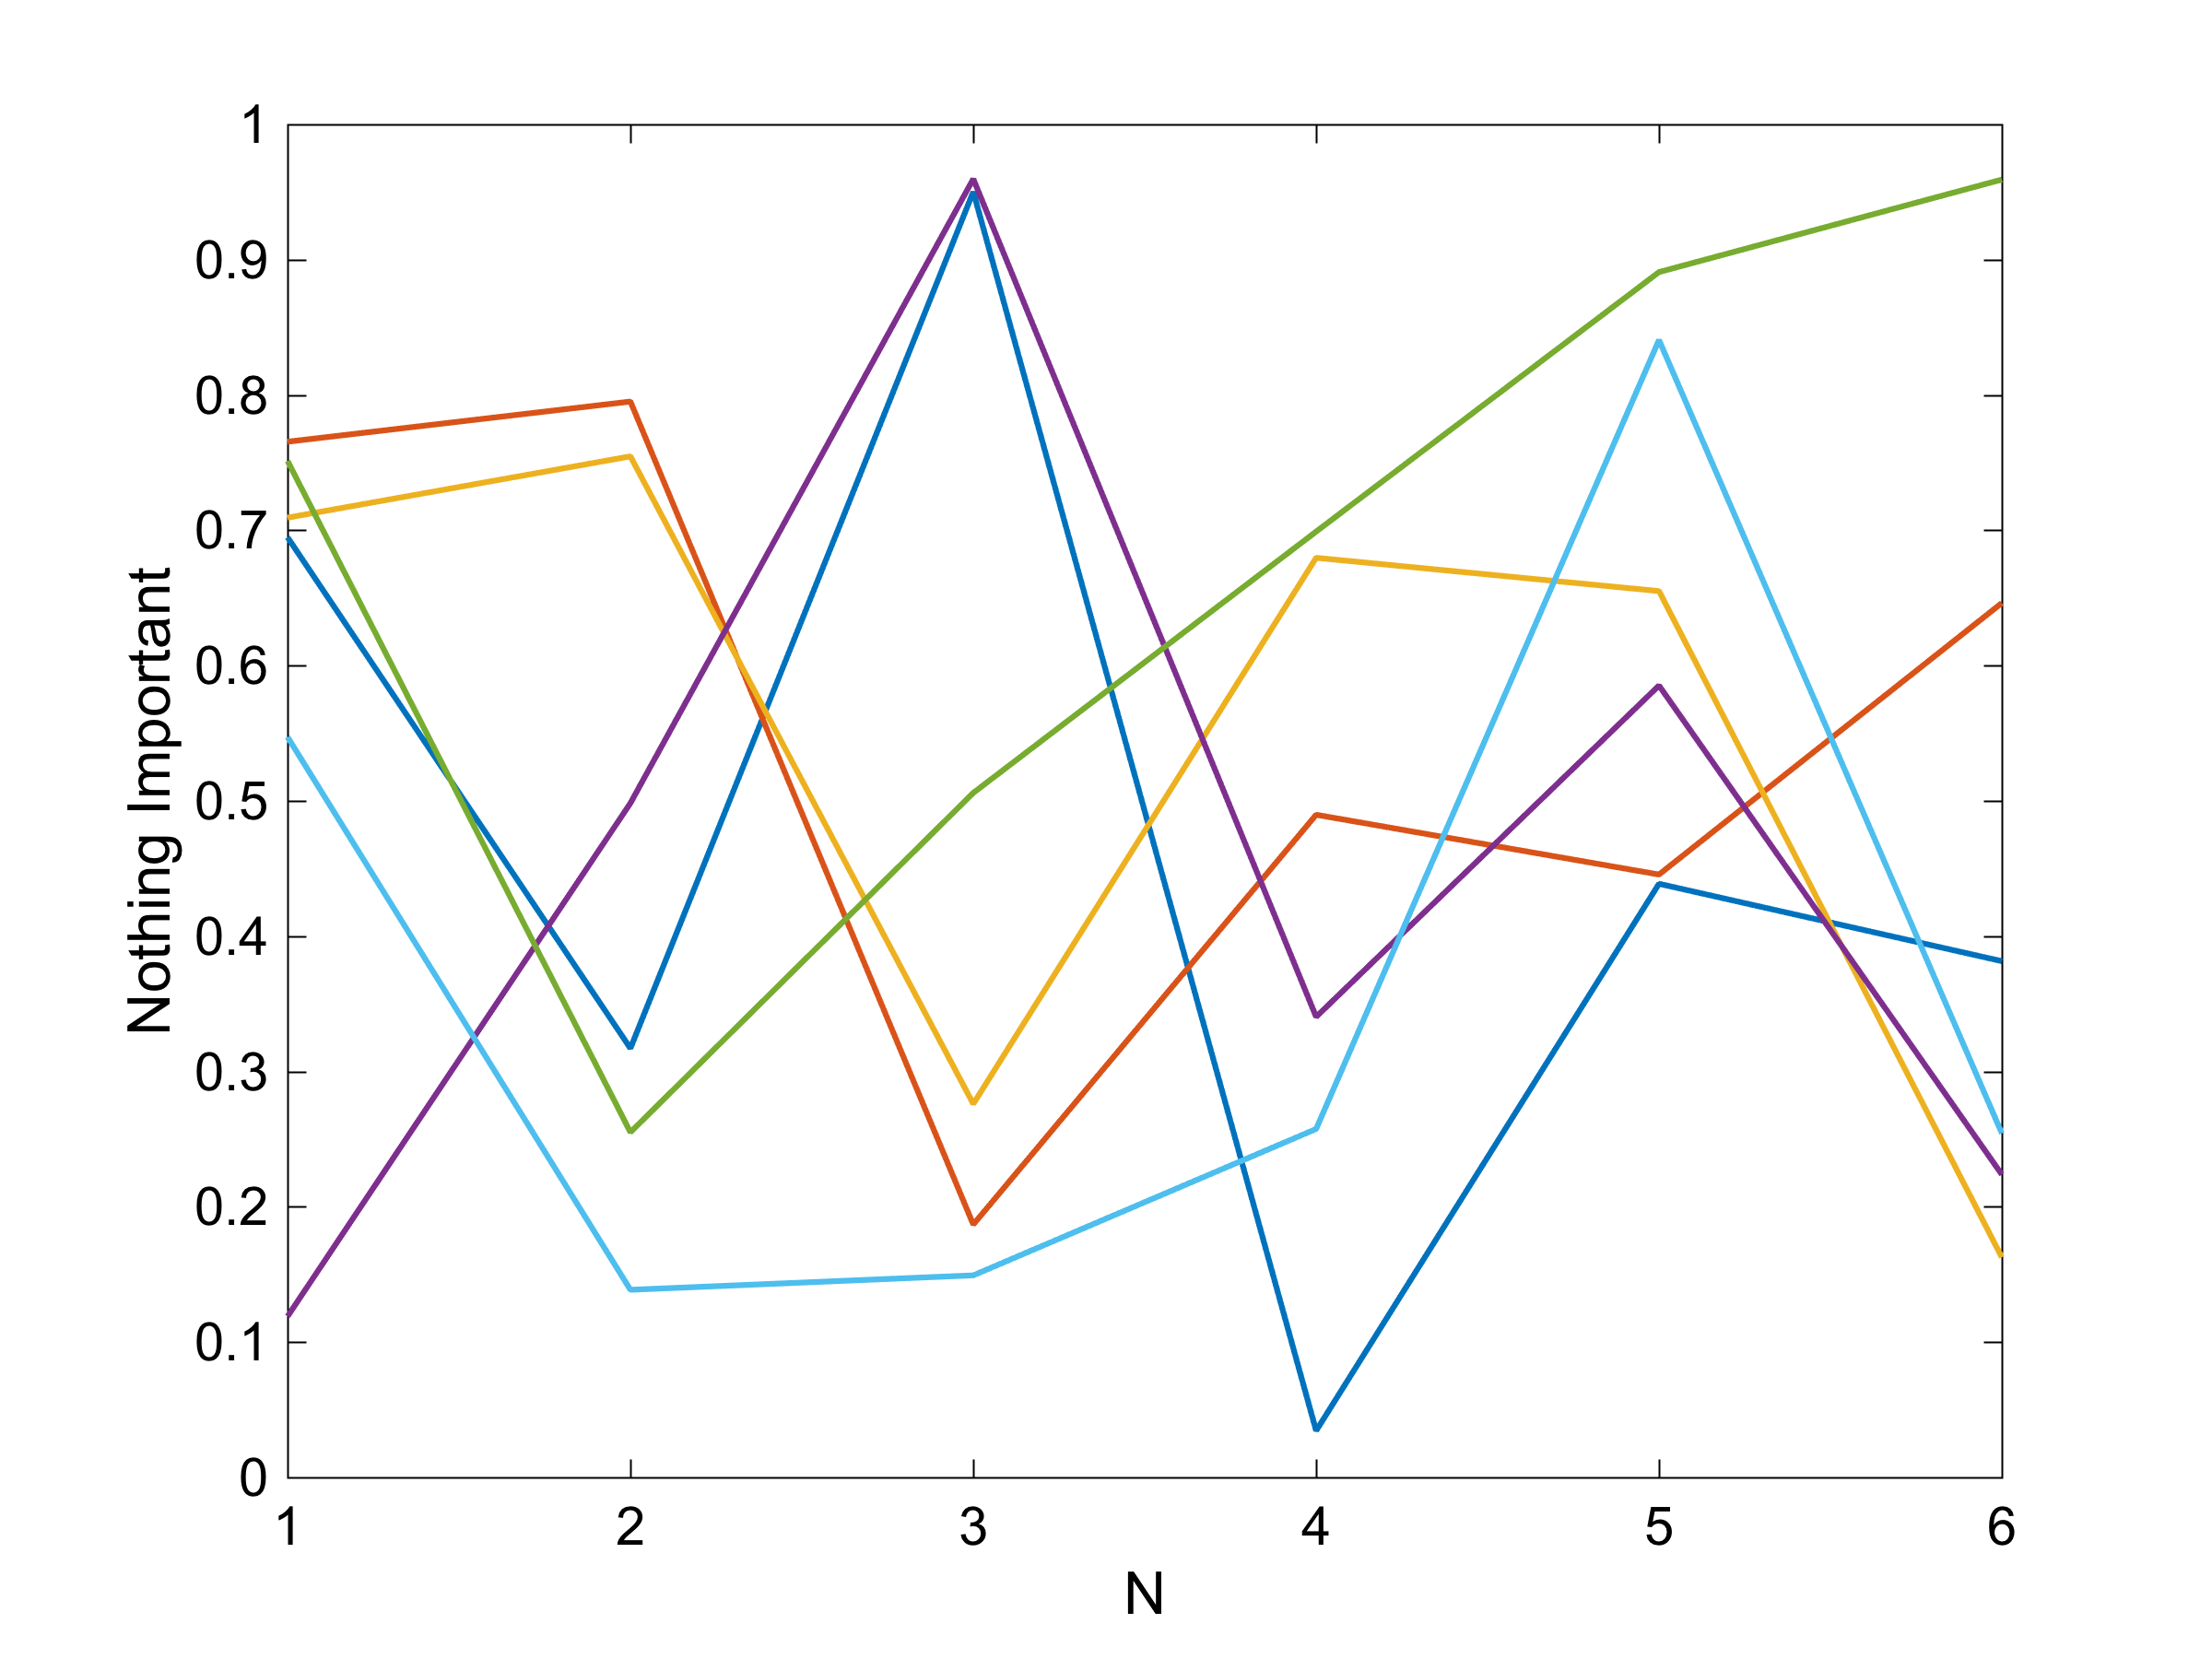
\includegraphics[width=0.85\textwidth,trim=10 10 10 10,clip]{sb_figure1}
\caption{Random plot for the sidebar. There isn't much to say here, as the results are random.\label{sb_fig1}}
\end{figure}

\begin{thebibliography}{10}
	\bibitem[S1]{S1} Random reference number one generated for a sidebar, 2016
	\bibitem[S2]{S2} Random reference number two generated for a sidebar, 2016
\end{thebibliography}

\newpage
\processdelayedfloats % place sidebar endfloats here
\clearpage


%%%%%%%%%%%%%%%%%%%%%%%%%%%%%%%%%%%%%%%%%%%%%%%%
%%%%%%%%%%%%%%%%%%%%%%%%%%%%%%%%%%%%%%%%%%%%%%%%
%%%%%%%%%%%%%%%%%%%%%%%%%%%%%%%%%%%%%%%%%%%%%%%%
\clearpage
\section[Use of Hyphens]{Sidebar: Use of Hyphens}
\label{sb:UseofHyphens}
       			
Note the spelling of these words as single words with no hyphen:  aeroelastic, aeroservoelastic, aimpoint, allpass, axisymmetric, backup, bandpass, bandlimited, bloodstream, breakpoint, buildup, colocated, coprime, countdown, counterclockwise, counterintuitive, counterproductive, crossover, cutoff, deadbeat, deadzone, drivetrain, electromechanical, feedback, feedforward, feedthrough, flyby, gearbox, geartrain, handheld, hardwired, highpass, ingoing, inline, interagent, interarrival, interrelated, liftoff, lightweight, longstanding, lookup, lowpass, multidimensional, multidisciplinary, multilayer, multilevel, multimode, multimodel, multiobjective, multipath, multirate, multiscale, multistage, multistep, multivehicle, narrowband, nonadaptive, nonadditive, noncausal, noncolocated, nonconservative, noncontact, nonconvex, nondestructive, nondeterministic, nondissipative, nonempty, nonequilibrium, nonessential, nonferrous, nonholonomic, nonideal, noninvasive, nonlinear, nonlocal, nonminimum, nonnegative, nonoverlapping, nonrepeating, nonsquare, nonstandard, nonstationary, nontrivial, nonuniform, nonzero, offboard offline, offset, offshoot, offsite, onboard, ongoing, online, onsite, outgoing, overcrowded, overparameterized, passband, piecewise, powertrain, preset, reinvent, rewritten, rolloff, rollover, rollup, roundoff, scaleup, setpoint, setup, shutdown, sideslip, speedup, spinup, startup, subdivision, suboptimal, subregion, subsection, substep, subsystem, swingby, swingup, teamwork, testbed, tradeoff, unidirectional, warmup, workpiece, worldwide.
       	
%\clearpage
%\section{Procedures}
%Once a conditional acceptance decision is communicated, electronic submission of all materials listed below is required.  Paper copies are not required.
\bee
\item Single-column PDF version of your entire article, including biographies, with each figure and its caption on a separate page at the end of the article.  
Be sure that your figure captions include a statement of permission for all copyrighted material.\\  \textit{Remember:}  It is your responsibility to obtain permission to use copyrighted images.  

\item Source files (with possible BIB file) for the article in Word or Latex.  The files should include all references, sidebars, figures, and captions.  

\item Designate the corresponding author, and include the complete email address for the corresponding author only on the first page.  

\item A separate, clearly labeled file for each figure. and each filename should include the corresponding figure number.
Acceptable file formats are tiff, eps, ps, pdf, and jpg (eps and pdf preferred).  Name these figure files ``\verb!figure1_other_text.eps!''.  Figures embedded in Word documents or PowerPoint slides cannot be extracted and are not useful.  

\item A signed copyright form.  You must print, sign, scan, and email the first page of the IEEE copyright form.  Only one author needs to sign. The copyright form is at\\ \url{http://www.ieee.org/publications_standards/publications/rights/copyrightmain.html.}

\item Email photos of all of the authors, preferably within a control or laboratory setting, or at a control conference. Other options are interesting photos such as while traveling, skiing, hiking, sailing, or portrait photos. Please label these files with the intended caption. For example use the file name \verb!Jonathan_P_How_skiing_in_New_Hampshire.jpg!.

\item Short ($\sim$1 paragraph) summary/abstract highlighting the article's main 
contributions that can be used for material in the ``About this Issue'' section of the IEEE CSM.

\item Proposed artwork for IEEE CSM front cover related to your article - see past issues for inspiration and guidance.
\eee
%\vspace*{-.25in} 
Zip up all of these files (source, complete PDF of the entire article, figure files, signed copyright form, author photos, one paragraph summary, proposed cover art) into a folder labeled in the format 
\verb!CSMXX-00YY_correspondingauthorlastname_FINAL,! 
where “XX-00YY” refers to the official IEEE CSM number of your paper, as in “CSM16-0037JonesFINAL.”

%\vspace*{-.25in} 

\bc
\textbf{Required electronic materials include the following items to be sent to the Editor-in-Chief Jonathan P. How (how.jonathan@gmail.com)
}\ec

\newpage
\section{Author Biography}
Insert the author bios here.
%\input{author_how}

\end{document}